\section{Dashboard}
  L' header della dashboard è uguale come struttura per ogni tipo di utenza. Su di essa troviamo un link che porta alla modifica dei dati personali, chiamato \texttt{profilo} e un link \texttt{Esci}, che effettua il logout dal sistema.



\subsection{Struttura}
    \begin{figure}[H]
        \centering
        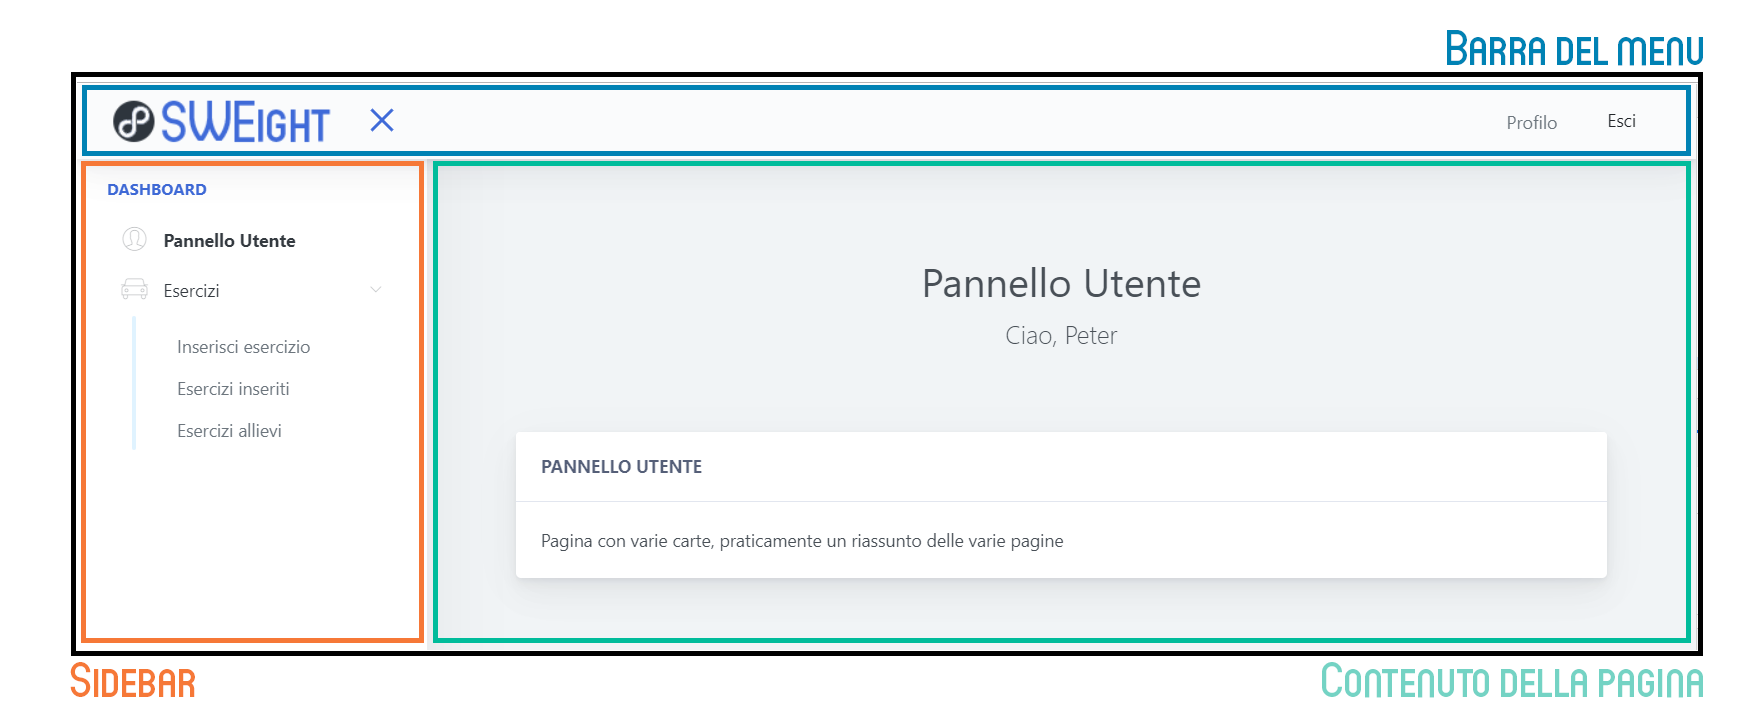
\includegraphics[width=17cm]{sez/img/istruzioni/dashboardMod.png} 
        \caption{Svolgimento esercizio}\label{fig:1}
    \end{figure}
  Questa sezione serve per definire i termini con cui chiamare gli elementi che compongono la pagina dell'applicazione.
    Componenti principali:
    \begin{itemize}
        \item Barra del menu;
        \item {Sidebar}\ped{G};
        \item Contenuto della pagina.
    \end{itemize}


\subsection{Autenticazione}
    \subsubsection{Registrazione}
    	\begin{figure}[H]
        	\centering
        	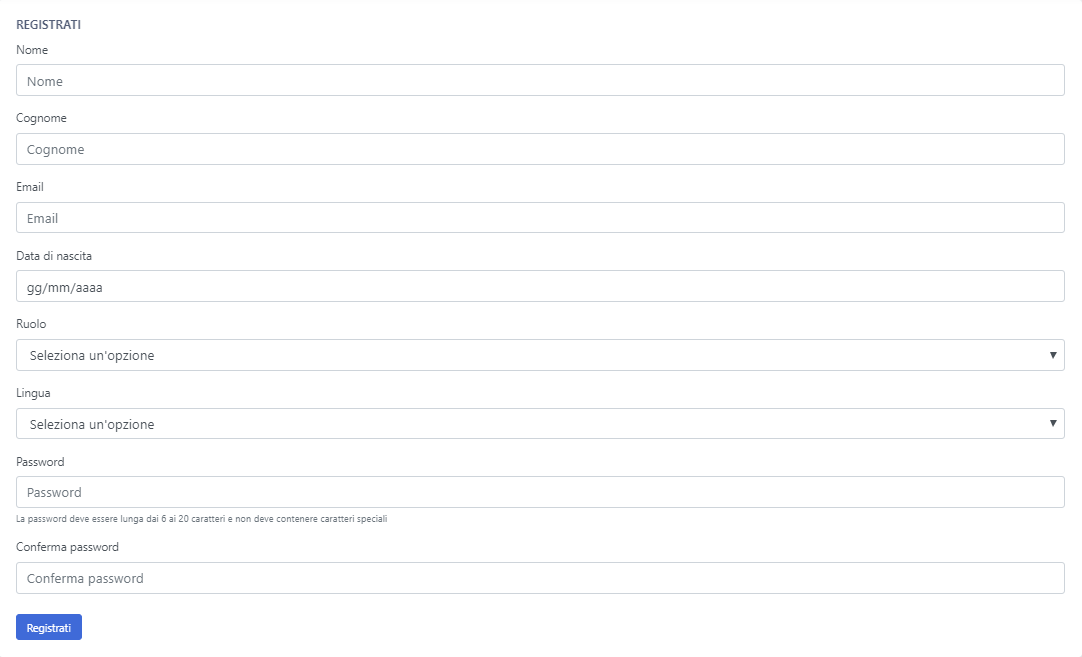
\includegraphics[width=1\linewidth]{sez/img/autenticazione/formRegistrazione.PNG} 
        	\caption{Form per la registrazione}\label{fig:1}
    	\end{figure}
	  Se non si è ancora registrati è possibile farlo cliccando sul button \textit{Registrati} presente nella barra del menu. Una volta compilato il form sarà possibile accedere alla piattaforma come utente autenticato. Se si sceglie come ruolo \textit{sviluppatore} sarà necessario attendere una conferma da parte dell'amministratore prima di poter accedere. I dati sono tutti obbligatori e la form visualizzata sarà la seguente.

    \subsubsection{Login}
    	\begin{figure}[H]
        	\centering
        	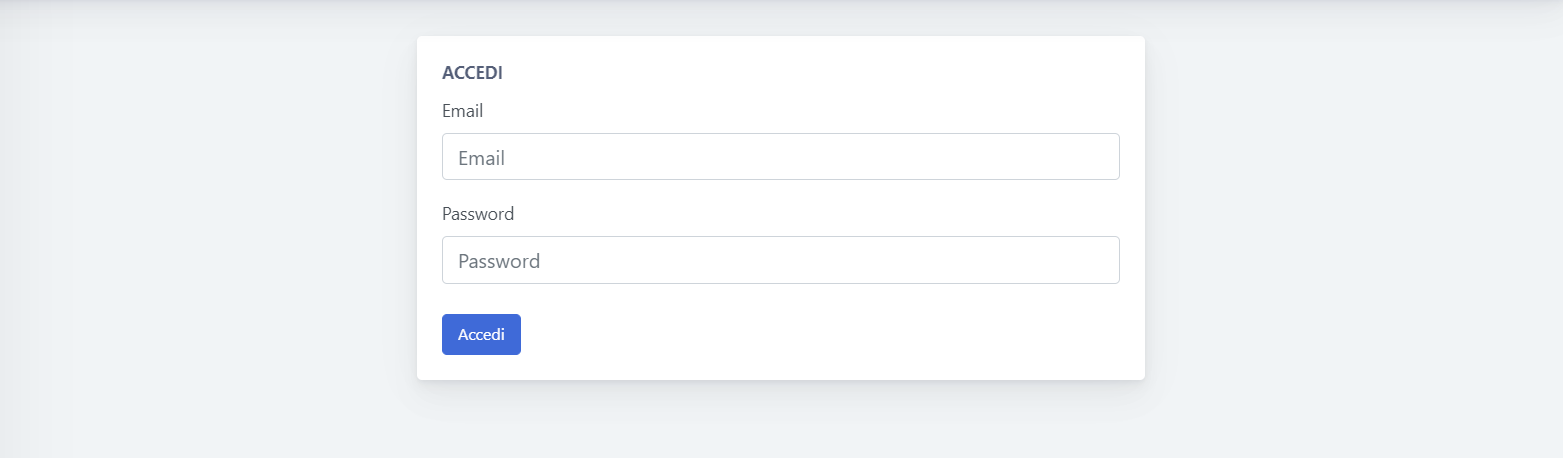
\includegraphics[width=1\linewidth]{sez/img/autenticazione/formAccedi.PNG} 
        	\caption{Dati per effettuare l'accesso}\label{fig:1}
    	\end{figure}
 	  Dopo aver effettuato la registrazione si accede cliccando su \textit{Accedi} nella barra del menu. Si accede inserendo email e password.
    
    \subsubsection{Logout}
    Per effettuare il {logout}\ped{G} si deve cliccare su la voce \textit{Esci} dalla barra del menu. Esso permette all'utente  di finire la propria sessione.


% UTENTE AUTENTICATO
\subsection{Utente autenticato}

    \subsubsection{Studente}
      Lo studente è l'utente che può svolgere esercizi, con correzioni automatiche oppure con correzioni degli insegnanti.
        \paragraph{Sidebar} \mbox{}\\ \\
          Sidebar dello studente presenta le seguenti voci:
            \begin{itemize}
                \item Pannello utente;
                \item Esercitazione libera;
                \item Compiti per casa;
                \item Esercizi svolti;
                \item I tuoi voti.
            \end{itemize}
            
            
            
            
            
            
        \paragraph{Pannello utente}\mbox{}\\ \\
          SCREEN NON DISPONIBILI
          Il pannello utente è un riassunto di tutti i progressi e le attività svolte dallo studente.
          Contenuto presente all'interno della pagina:
        	\begin{itemize}
        		\item Progressi;
        		\item Traguardi;
        		\item Traguardo corrente;
        		\item Prossimo traguardo;
        		\item Valutazioni;
        		\item Esercizi recenti;
        		\item Insegnanti preferiti.
        	\end{itemize}
        
        
               
	\newpage
        \paragraph{Esercitazione libera}\mbox{}\\ \\        
        	\begin{figure}[H]
                \centering
                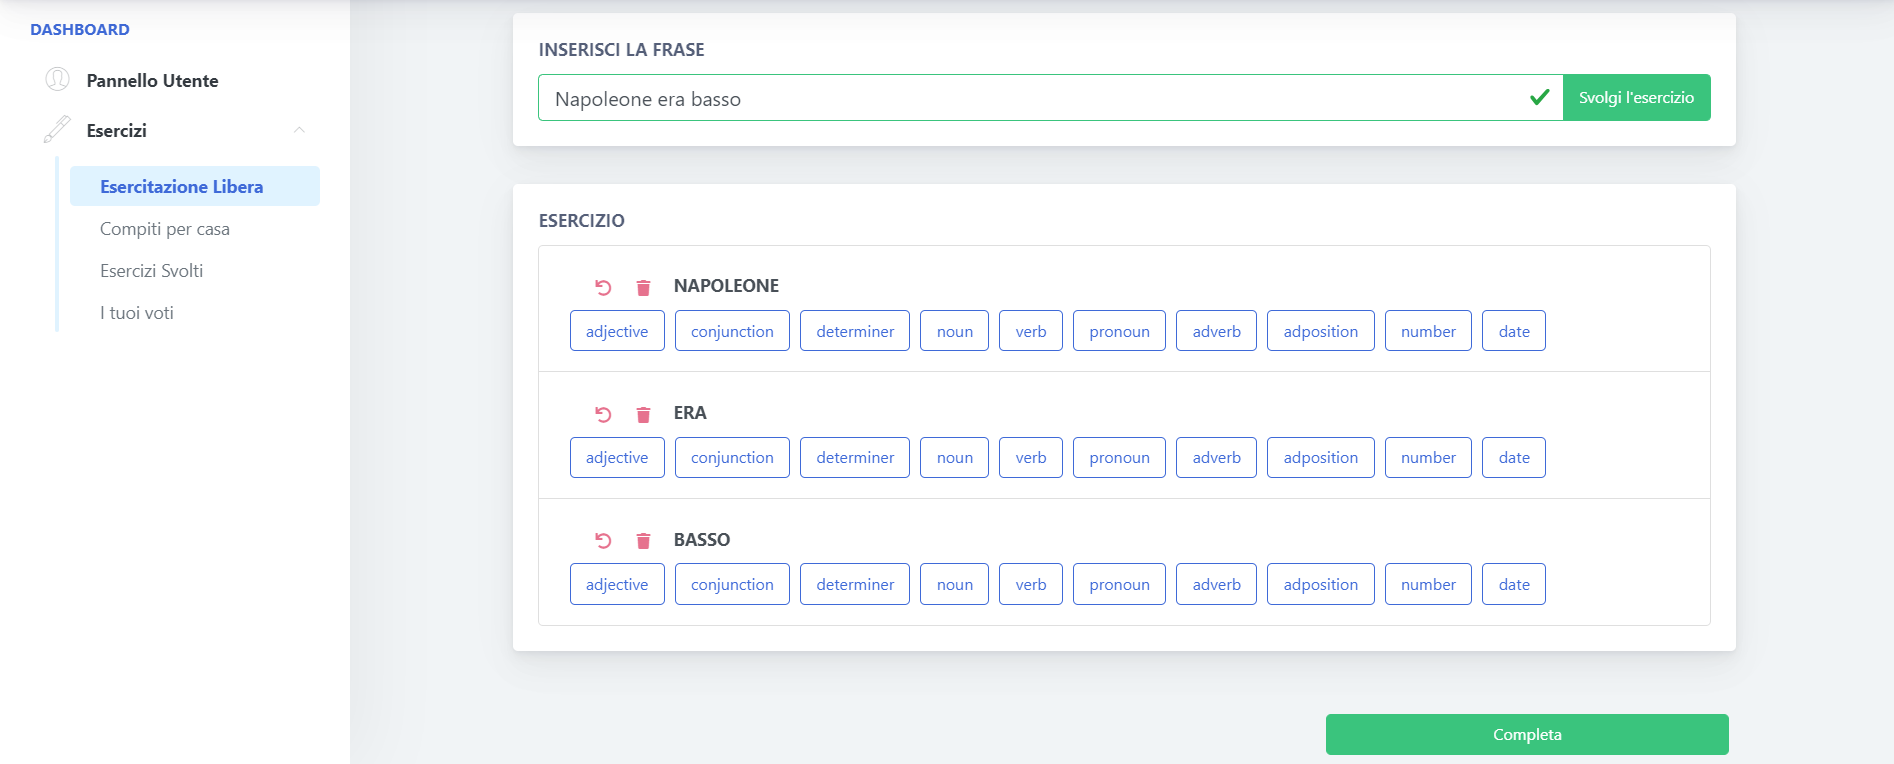
\includegraphics[width=17cm]{sez/img/studente/esercitazioneLiberaEsegui.PNG} 
                \caption{sidebar dello stidente}\label{fig:1}
        	\end{figure}
          In questa sezione si svolge l'esercizio inserendo nel form la frase che 
        si preferisce. Se la frase non è stata inserita da nessun insegnante la 
        correzione sarà generata automaticamente.
        \\ Svolgimento:
        	\begin{enumerate}        
            	\item Scrivi la frase che vuoi analizzare dentro al form;
            	\item Clicca su \textit{svolgi esercizio};
            	\item Svolgi l'esercizio e clicca \textit{completa}.
        	\end{enumerate}
           In questa sezione è possibile visualizzare gli esercizi che sono stati assegnati dall'insegnante dove può scegliere che esercizio svolgere.
  
        
        
        
        
        
  		\paragraph{Compiti per casa}\mbox{}\\ \\
 
        	\begin{figure}[H]
            	\centering
            	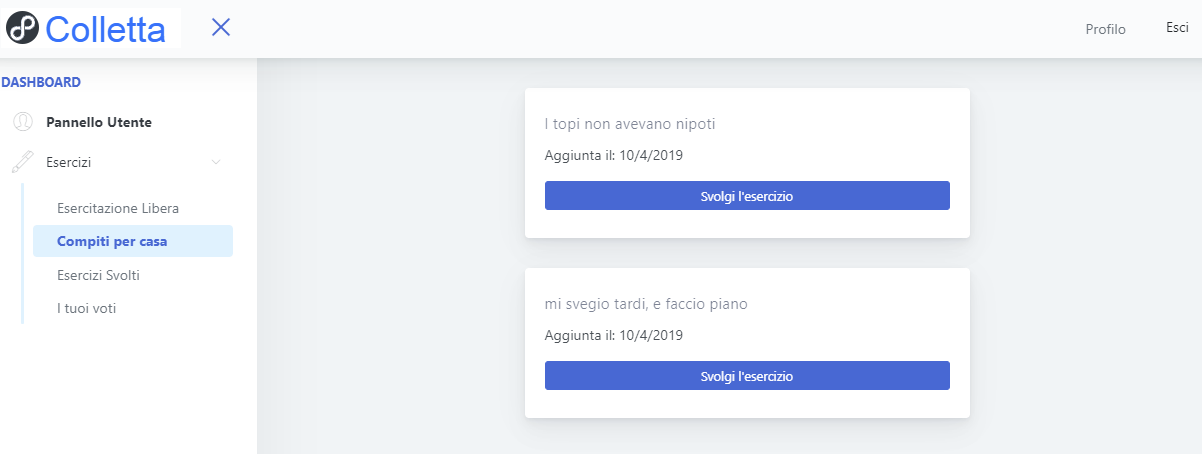
\includegraphics[width=17cm]{sez/img/studente/compitopercasa.PNG} 
            	\caption{Studente: Scelta esercizio da risolvere}\label{fig:1}
        	\end{figure}

		  Lo studente sceglie l'esercizio da svolgere tra quelli che sono stati assegnati cliccando su \textit{Svolgi l'esercizio}.   
       
        	\begin{figure}[H]
            	\centering
            	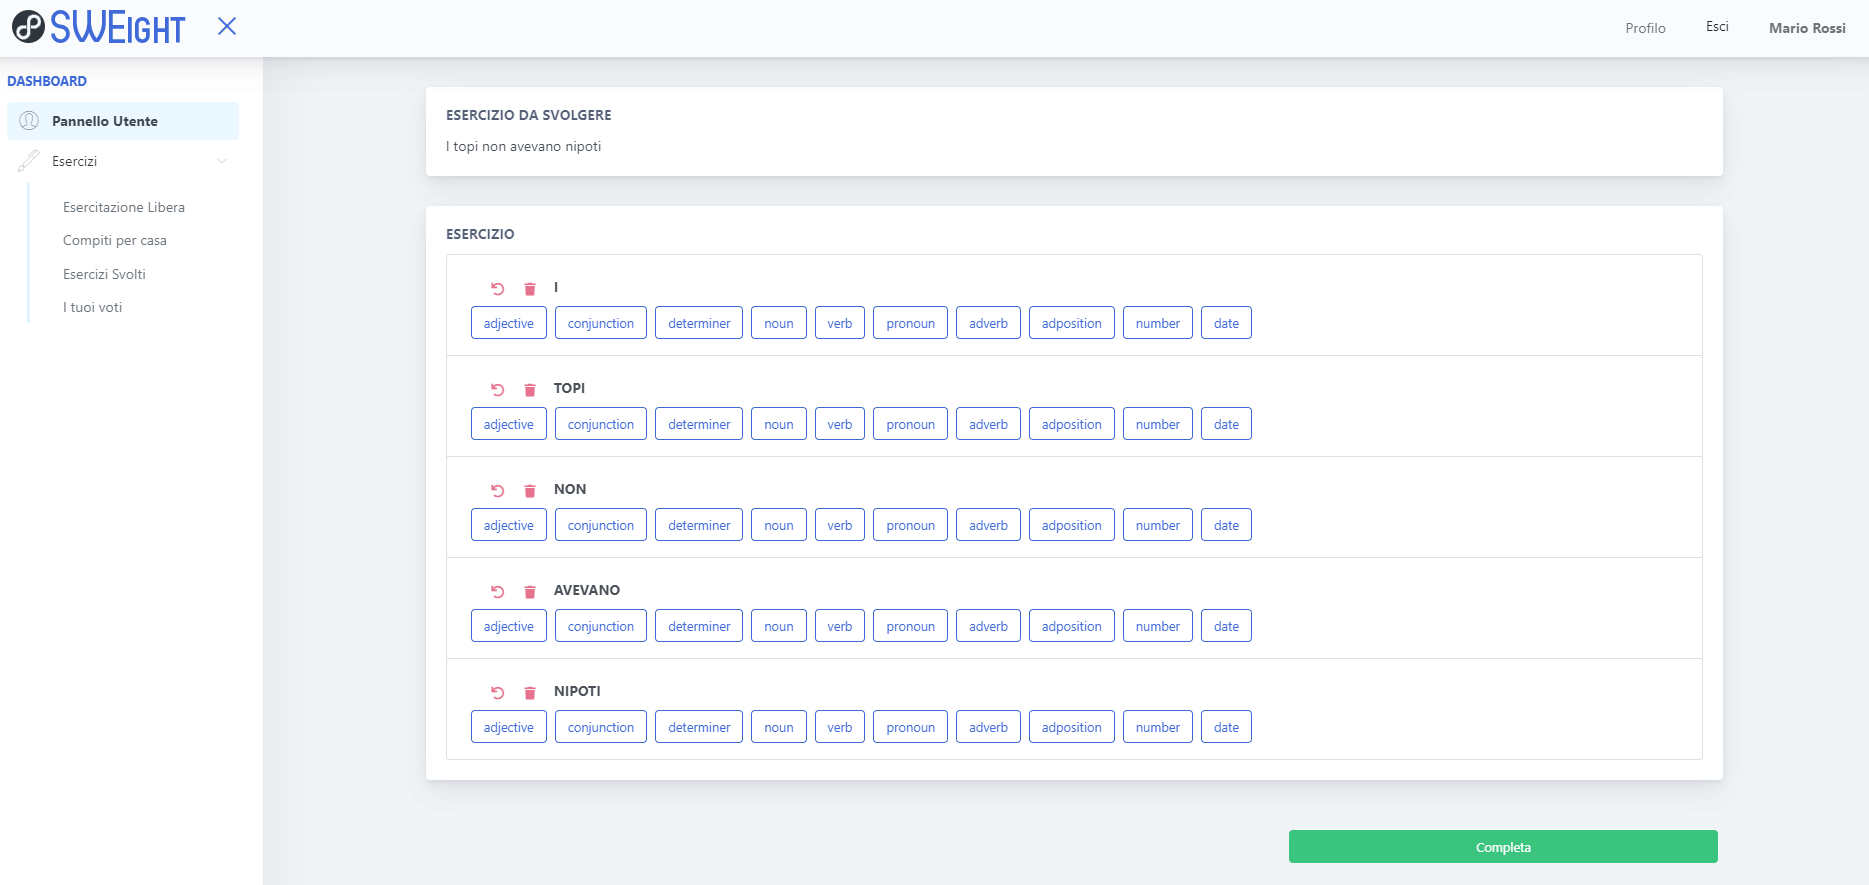
\includegraphics[width=17cm]{sez/img/studente/svolgimentoesercizio.PNG} 
            	\caption{Studente: Svolgimento esercizio}\label{fig:1}
        	\end{figure}   
           Scelto l'esercizio va svolto dove lo studente ha la  possibilità di tornare indietro di un passo, se ha assegnato alla parola un tag sbagliato o di cancellate completamente tutti i tag e ricominciare da capo parola per parola. Infine cliccando \textit{Completa} invia la sua soluzione che verrà controllata e valutata dall'insegnante.
        
        
        
        
        \paragraph{Esercizi svolti}\mbox{}\\ \\
        	\begin{figure}[H]
            	\centering
            	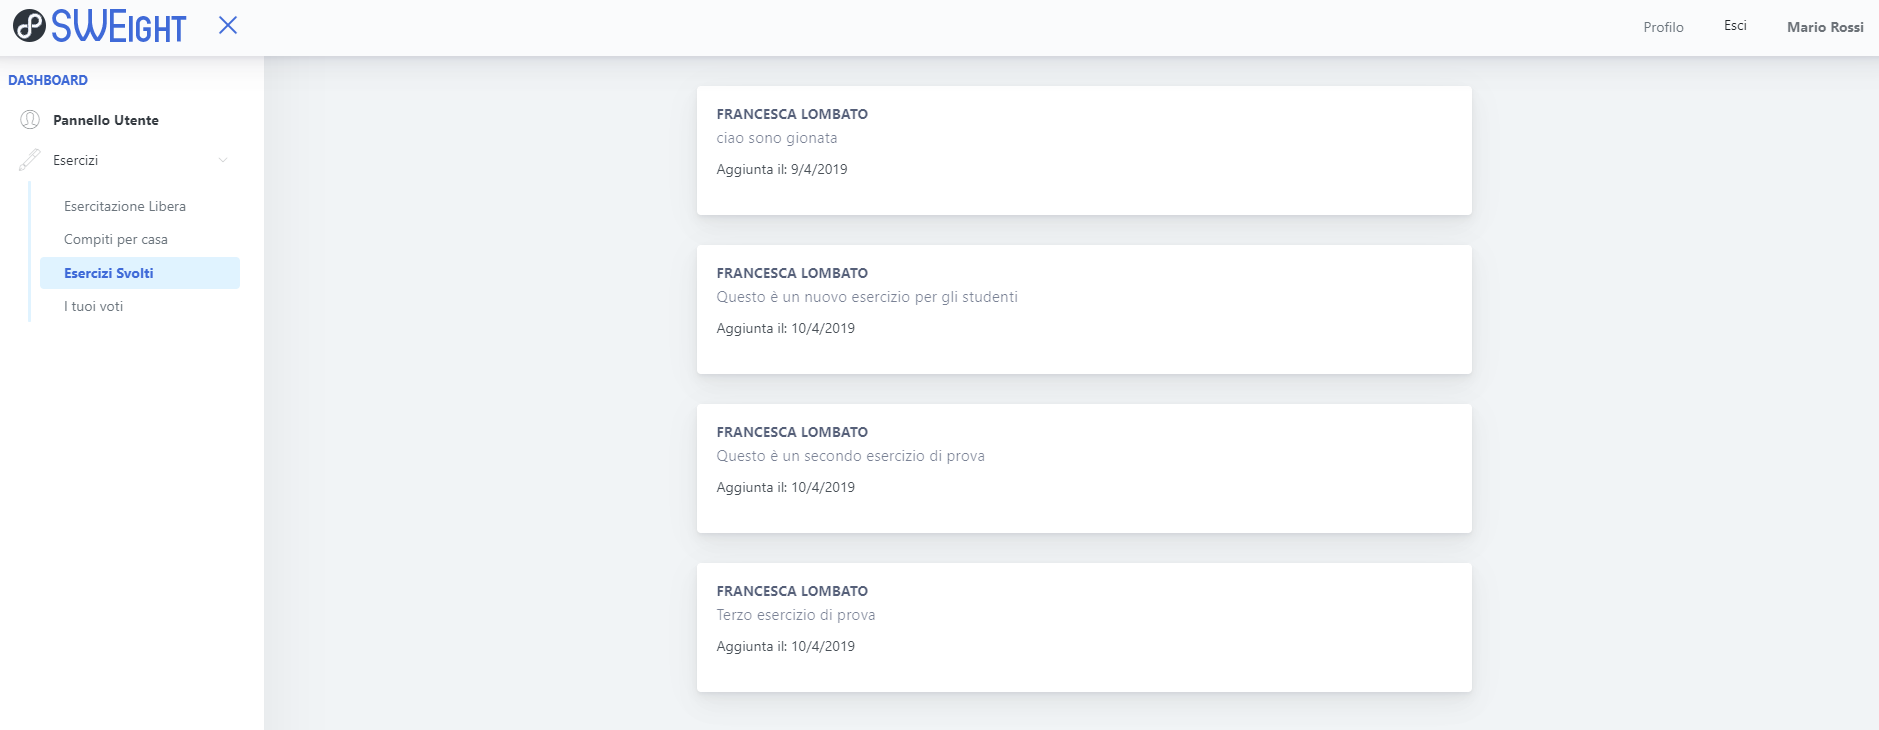
\includegraphics[width=17cm]{sez/img/studente/esercizisvolti.PNG} 
            	\caption{Studente: Storico esercizi svolti}\label{fig:1}
        	\end{figure}
          In questa sezione è possibile visualizzare  lo storico degli esercizi che sono stati svolti.
        
        
        
        
        \paragraph{I tuoi voti}\mbox{}\\ \\
          SCREEN NON DISPONIBILI
          In questa sezione è possibile visualizzare i voti....
        
        
        
        
        
\newpage
    \subsubsection{Insegnante}
      L'insegnante è l'utente che può inserire esercizi e assegnarli.
        \paragraph{Sidebar}\mbox{}\\ \\
          Sidebar dell'insegnante presenta le seguenti voci:
        	\begin{itemize}
            	\item Pannello utente;
            	\item Inserisci esercizio;
            	\item Esercizi inseriti;
            	\item Esercizi allievi.
        	\end{itemize}
        
        
        
        \paragraph{Pannello utente}\mbox{}\\ \\
          Il pannello utente è un riassunto di tutti i progressi e le attività.
         \\Contenuto presente all'interno della pagina:
        	\begin{itemize}
        	\item Storico esercizi inseriti; 
        	\item Esercizi recenti svolti dagli studenti;
        	\item Elenco propri studenti;
        	\item Elenco classi studenti.
        	\end{itemize}
        
        
        
        
        \paragraph{Inserisci esercizio}\mbox{}\\ \\
          Questa sezione da la possibilità all'insegnante di inserire un esercizio.
        	\begin{figure}[H]
            \centering
        	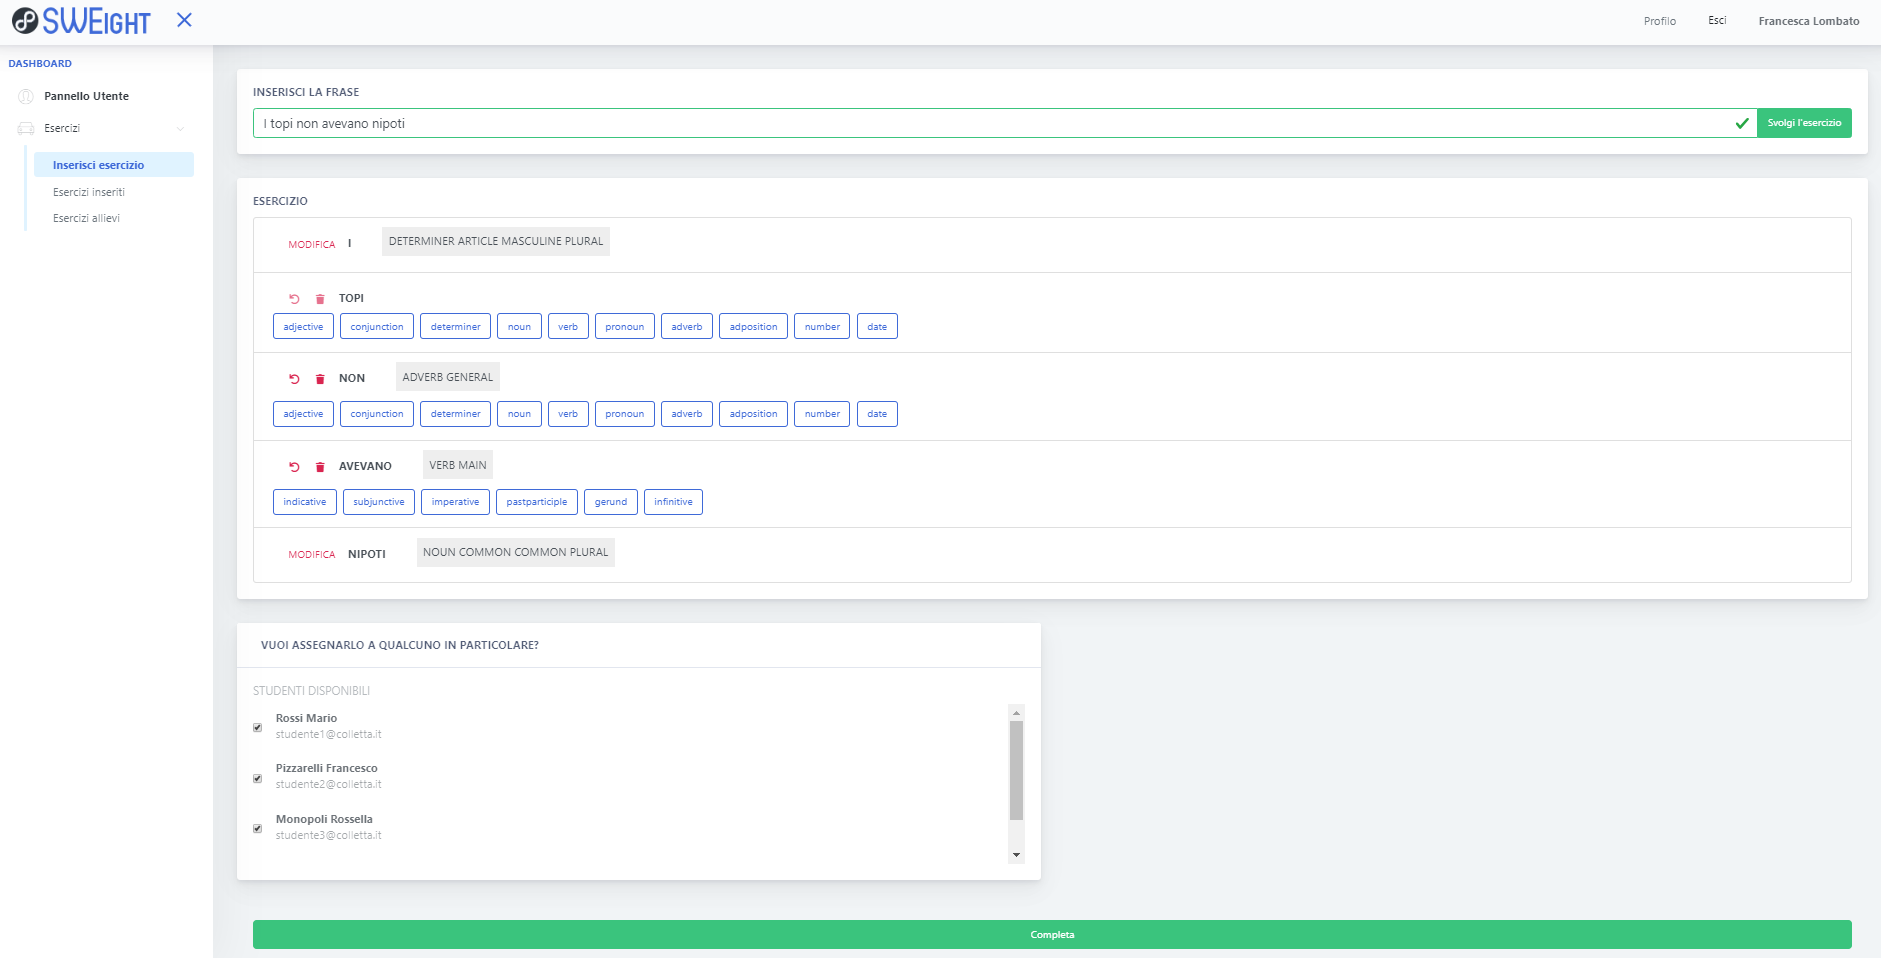
\includegraphics[width=17cm]{sez/img/insegnante/inserisciEsercizio.PNG} 
            \caption{Insegnante: Inserisci esercizio}\label{fig:1}
        	\end{figure}
        
          Dopo aver inserito la frase verrà visualizzata la correzione automatica. Se ritenuta errata c'è la possibilità di modificare la soluzione cliccando su \textit{Modifica}. Durante lo svolgimento del esercizio l'insegnante ha la possibilità di tornare indietro di un passo, se ha assegnato alla parola un tag sbagliato o di cancellate completamente tutti i tag e ricominciare da capo parola per parola. Finita la correzione l'insegnate ha la possibilità di assegnare l'esercizio a uno studente e cliccando \textit{Completa} verrà aggiunto nel database.
        
        
        
        \paragraph{Esercizi inseriti}\mbox{}\\ \\
        SCREEN NON DISPONIBILI
        
          Questa sezione permette di visualizzare tutti gli esercizi inseriti.
        
        
        
        
        \paragraph{Esercizi allievi}\mbox{}\\ \\
        SCREEN NON DISPONIBILI
        
          In questa sezione verranno visualizzati gli esercizi svolti dagli studenti che posso essere corretti e può dare un voto.
        
        
        
        
	\newpage
    \subsubsection{Sviluppatore}
    
    	\paragraph{Sidebar}\mbox{} \\ \\
    	  Sidebar dello sviluppatore presenta le seguenti voci:
    		\begin{itemize}
    		\item Pannello utente;
    		\item Pannello sviluppatore.
    		\end{itemize}
    
    
    
    
    	\paragraph{Pannello utente}\mbox{}\\ \\
    	  Contenuto presente all'interno della pagina:
        	\begin{itemize} 
        	\item Esercizi disponibili per il download;
        	\item Modelli disponibili per il download;
        	\item Filtri per raffinare il contenuto per il download;
        	\end{itemize}




    	\paragraph{Pannello sviluppatore}\mbox{}\\ \\
    		\begin{figure}[H]
			\centering
			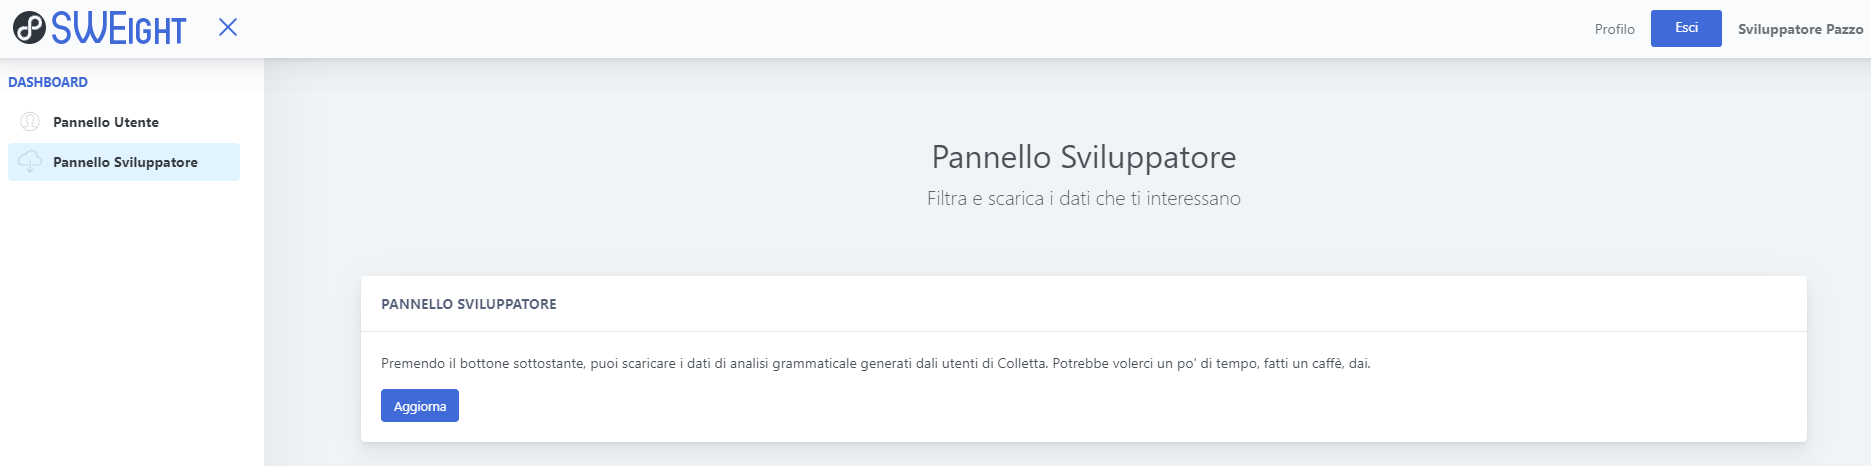
\includegraphics[width=17cm]{sez/img/sviluppatore/datipronti.PNG}
			\caption{Sviluppatore: Dati pronti per il download}\label{fig:1}
			\end{figure}
		  Possibilità per fare il download dei dati attualmente disponibili.




	\newpage
	\subsubsection{Amministratore}
		\paragraph{Sidebar}\mbox{}\\ \\
		  Breve guida per l'amministratore che amministra gli utenti all'interno della piattaforma. Sidebar dell'amministratore presenta le seguenti voci:
			\begin{itemize}
			\item Pannello utente;
			\item Sviluppatori;
			\item Utenti.
			\end{itemize}



		\paragraph{Pannello utente}\mbox{}\\
		  Accesso rapido a:
			\begin{itemize}
			\item statistiche;
			\item cose per amministratori;
			\item strumenti;
			\item bla bla.
			\end{itemize}
			  MANCA SCREEN.




		\paragraph{Sviluppatori}\mbox{}\\ \\
			\begin{figure}[H]
			\centering
			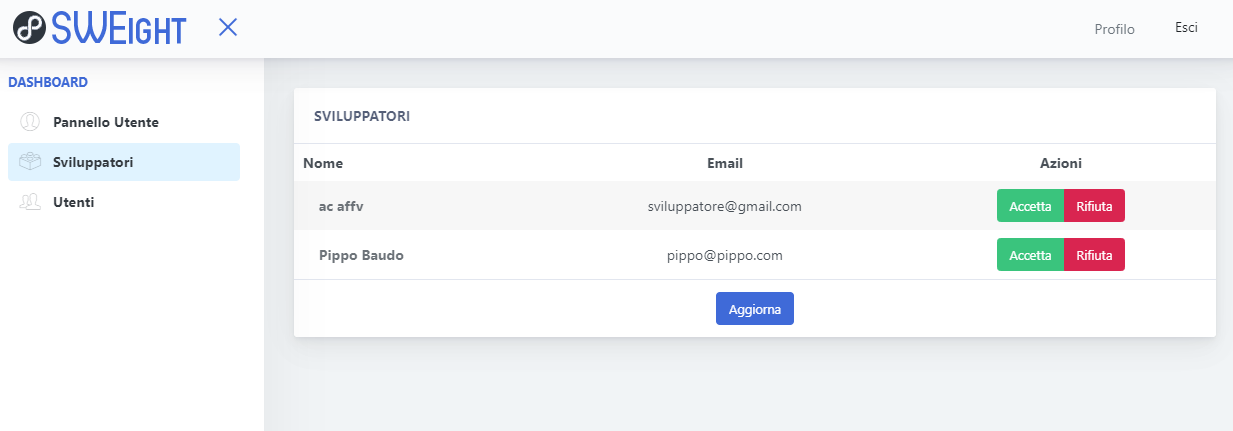
\includegraphics[width=17cm]{sez/img/amministratore/conf_ric_svil.PNG}
			\caption{Amministratore: Conferma richieste}\label{fig:1}
			\end{figure}
		  Le richieste da parte degli sviluppatori per accedere ai dati.


		\paragraph{Utenti}\mbox{}\\ \\
			\begin{figure}[H]
			\centering
			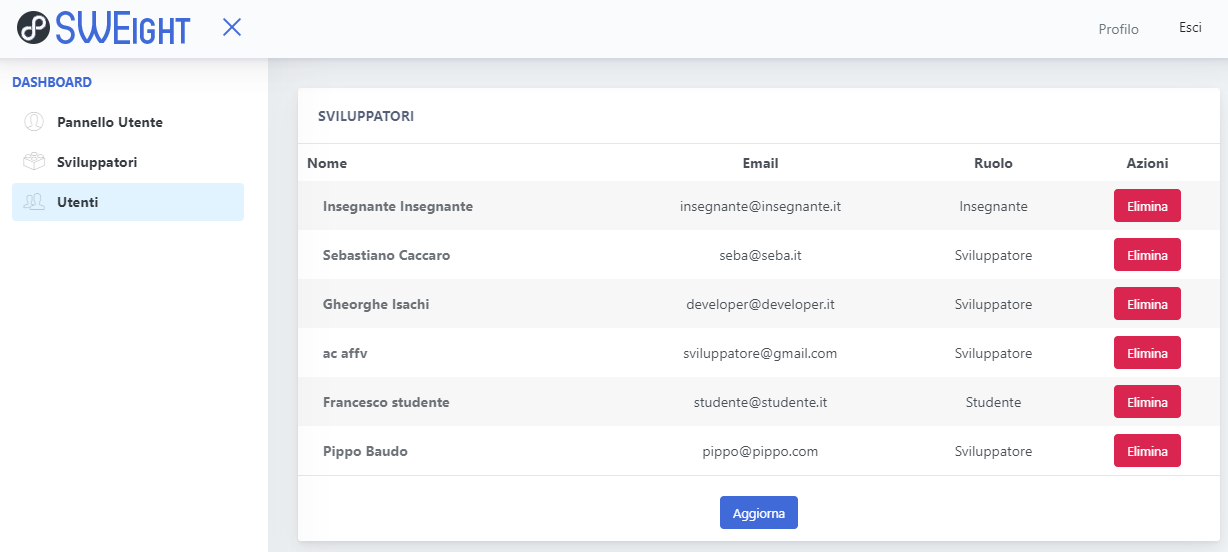
\includegraphics[width=17cm]{sez/img/amministratore/gestisciutenti.PNG}
			\caption{Amministratore: Gestione utenti}\label{fig:1}
			\end{figure}
		  La lista degli utenti presenti e la loro gestione.
